\pdfminorversion=7
\documentclass[../main.tex]{subfiles}

\begin{document}
\ifx\chapincluded\undefined
  \begin{refsection}[main-bib]
 \fi

 \chapter{Research Contributions}
\label{chap:rcontrib}

The research contributions of this thesis are presented in five
articles. The first four
(\Cref{chap:cal-paper,chap:pact-paper,chap:wosc-paper,chap:hpca-paper})
are published and the final paper (\Cref{chap:eurosys-paper}) is
pending review at the time of thesis submission. In this chapter, we
summarize the contributions of each paper and contextualize the papers
prior work. The rest of this chapter summarizes our research contributions starting from the research directions introduced in \Cref{sec:res-overview}.


\section{Contribution overview}

\subsection{Research Direction A: Hardware approaches to optimizing FaaS}
We present our results in two parts where the first partI
(\Cref{subsub:understanding}) covers the
background study, presented in Paper \liningfigures{A1} (\Cref{chap:wosc-paper}) and
the second part (\Cref{subsub:btbx}) describes BTB-X, the proposal for a
redesigned BTB proposal covered in Papers
\liningfigures{A2}, \liningfigures{A3} and \liningfigures{A4} (\Cref{chap:cal-paper,chap:pact-paper,chap:hpca-paper}).

\subsubsection{Understanding FaaS}
\label{subsub:understanding}
\paragraph{Motivation.} Function-as-a-service (FaaS) computing is a
rapidly growing cloud computing model that challenges fundamental
assumptions about the design of computing systems. In FaaS, the
fundamental unit of computation is a function, often with a very short
execution time. A FaaS function is loaded and spawned on demand when
it is needed to respond to an event. When the FaaS function has
finished execution, it is shut down and the resources allocated to its
execution are freed. This forces providers to co-schedule and queue
thousands of different functions for execution on the same processor
cores to maximize server utilization. This causes heavy execution
interleaving and means that if, for example. functions A and B are
executed in the sequence ABA, function A will not find much or any of
its microarchitectural state left behind the second time it is
executed. The thrashing of the microarchitectural state caused by
interleaved execution means that most invocations of FaaS functions
happen from a cold microarchitectural state. Recent work has noted
this and reported that the interleaved execution of FaaS functions
causes significant performance
deterioration~\cite{shahrad19_archit_implic_funct_servic_comput,lukewarm_serverless}. However,
no prior work investigates which specific properties FaaS functions
have that make them particularly vulnerable to the impact of state
thrashing. Is it, for example, dependent on the function code footprint size or the point where a function has a sufficiently long execution time to amortize the warm-up delay of the microarchitectural state?

\paragraph{Approach.}
To address this gap in the research, we evaluate FaaS functions
executed on a processor with warm and cold microarchitectural
states. We use a representative suite of FaaS functions consisting of
both real-world and synthetic workloads. Using synthetic workloads
allows us to modify specific parameters of interest in a controlled
way to determine their impact. To measure the impact of executing the
functions on a warm and cold microarchitectural state we execute the
functions in two modes: back-to-back and interleaved. In back-to-back
execution, the functions are executed repeatedly in a tight loop. In
the interleaved execution case, each invocation of a function is
interleaved with an invocation of a \emph{trhasher} function that
thrashes all existing microarchitectural state. The thrasher function
achieves this by performing two actions: \begin{inparaenum}[1)]
\item it invokes the x86 WBINVD
  instruction that writes back and invalidates the entire cache
  hierarchy of the processor package~\cite[Chapter 6]{intelmanual} and \item it runs a function that
  executes a long sequence of branches to thrash the state of
  the BTB and the branch predictor. \end{inparaenum} We measure
microarchitectural parameters using perf~\cite{perftool} and use the Top-Down
methodology~\cite{yasin14_top_down} for identifying specific
microarchitectural bottlenecks. For both the back-to-back and
interleaved executions we measured both the wall-clock running time of
the functions and relevant microarchitectural parameters.


To support our findings (presented below) we measure the code
footprint of each of the FaaS functions that we use in our
analysis. Doing this using a full microarchitectural simulator is a
slow and tedious process. Further, it is impossible to perform this
analysis statically since the dynamic instruction trace of a program
is only known at runtime. Therefore, we use a method described
in~\cite{splash2} that uses branch-record traces and a cache simulator
to estimate the code footprint of a program. The branch-record traces
show the branches taken by a program during execution. By feeding the
instruction code regions demanded by these branches through a cache
simulator, we can measure how big the cache has to be to fit the
entire code footprint of a program.  Specifically, the method changes
the size of the simulator cache until the observed miss-rate reaches
zero. When this is the case, the entire code footprint of the program
fits inside the cache.


\paragraph{Key Results.}
Our results show that two properties of a FaaS function impact how
sensitive it is to being executed on a cold microarchitectural state:
Its execution time and its code footprint. For example, the shortest
running function that we evaluate (0.25\,ms) shows a slowdown of
17\texttimes{} when executed on a processor with a cold
microarchitectural state. The longest running functions are largely
unaffected by microarchitectural state thrashing. Since 99\% of
real-world FaaS invocations run for more than
1\,ms~\cite{shahrad20_server_wild}, our results indicate that the
warm-up latency of microarchitectural structures is amortized for the
vast majority of FaaS functions.

Another important observation we make from our experiments is that the
real-world FaaS functions we evaluate are overwhelmingly front-end
bound. This is in line with similar observations made for general
server
workloads~\cite{ferdman12_clear_cloud,kanev15_profil,ayers19_asmdb}
and corroborates similar observations made for FaaS functions
specifically~\cite{lukewarm_serverless}. This strongly motivates
further research aiming to alleviate the front-end bottleneck to
optimize the execution of FaaS functions.



\subsubsection{A storage-efficient BTB organization for servers}
\label{subsub:btbx}

\paragraph{Motivation.}
The front-end bottleneck is a well-known and widely documented problem
affecting processors executing server
workloads~\cite{ailamaki99_dbmss_moder_proces,ferdman12_clear_cloud,kanev15_profil,ayers19_asmdb}. Compared
to other workload classes, server workloads pose particular challenges
for processor frontends due to their very large instruction
footprints. These footprints quickly overwhelm the capacities of the
\liningfigures{L1-I} and the Branch Target Buffer (BTB). To handle
this problem, computer architects have proposed a large number of
different approaches. In particular, \liningfigures{L1-I} prefetchers
are a highly effective way to alleviate the front-end bottleneck as
they help avoid the fill-latency that follows an \liningfigures{L1-I}
miss.  As detailed in~\Cref{sec:instr-delivery}, a particularly
effective class of instruction prefetchers are known as Fetch Directed
Instruction Prefetching
(FDIP)~\cite{reinman99_fetch_direc_instr_prefet}. Since FDIP rely on
the BTB to predict the control flow of a program and identify prefetch
candidates, having a BTB with sufficient capacity is of crucial
importance. By simply scaling the design of a conventional BTB design,
the capacity required for holding realistic branch working sets of
contemporary server workloads quickly become infeasible. To address
this, previous work observed that all branch targets within a page
share the same numbers and only differ in page offsets. Thus the page
number can be deduplicated by only storing it once in a dedicated
table and then replacing its use in a branch target address with a
pointer to that
table~\cite{seznec96_dont_use_page_number_point_it}. \textcite{soundararajan21_pdede}
extends this concept further by observing that several branch page
numbers share a common region number which can be deduplicated
further. The limitation of these approaches is that they add a level
of indirection to BTB lookups, adding complexity and increasing the
BTB access latency.


\paragraph{Approach.}

\begin{figure}[ht]
  \centering
  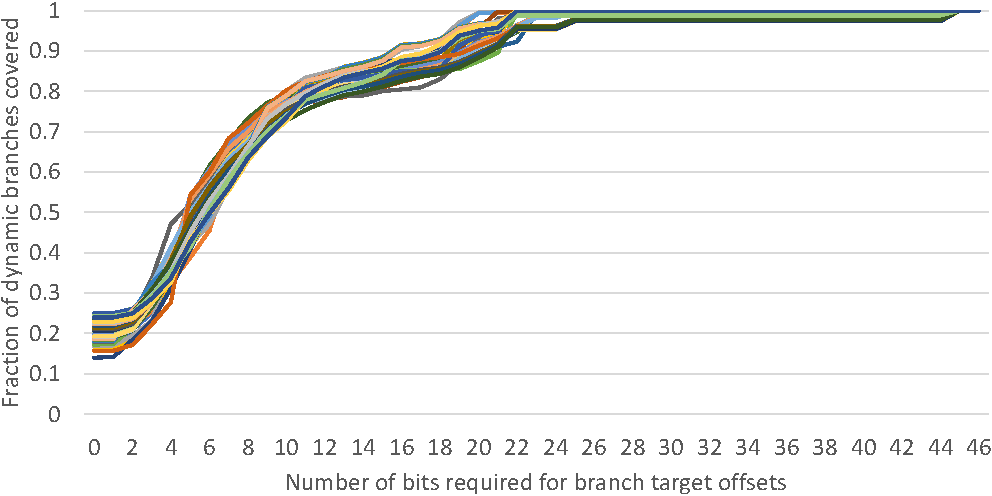
\includegraphics[width=0.8\textwidth]{figures/offset_distribution.pdf}
  \caption{\label{fig:offset-distr} Distribution of branch target offsets in the \liningfigures{IPC-1}~\cite{ipc1} workload traces}
\end{figure}

To gain a deeper understanding of the characteristics of branch
targets, we performed an analysis of the branch target offsets in a
large number of real-world workload traces released for the first
Instruction Prefetching Championship (\liningfigures{IPC-1})~\cite{ipc1}. A branch
target offset is the relative distance from a branch to its target. From this
analysis, shown in \Cref{fig:offset-distr}, we make the observation
that the vast majority of branches have targets very close to their
origin. For example, using just 19 bits we can represent the target
offsets of 90\% of all branches. This is significantly less than the
46 bits\footnote{This is assuming an Arm-64 architecture whre all
  instructions are 4 bytes long. Thus, we save the last two offset
  bits of the full 48-bit virtual address space.} required to store
the full target address.

\begin{figure}[ht]
  \centering
  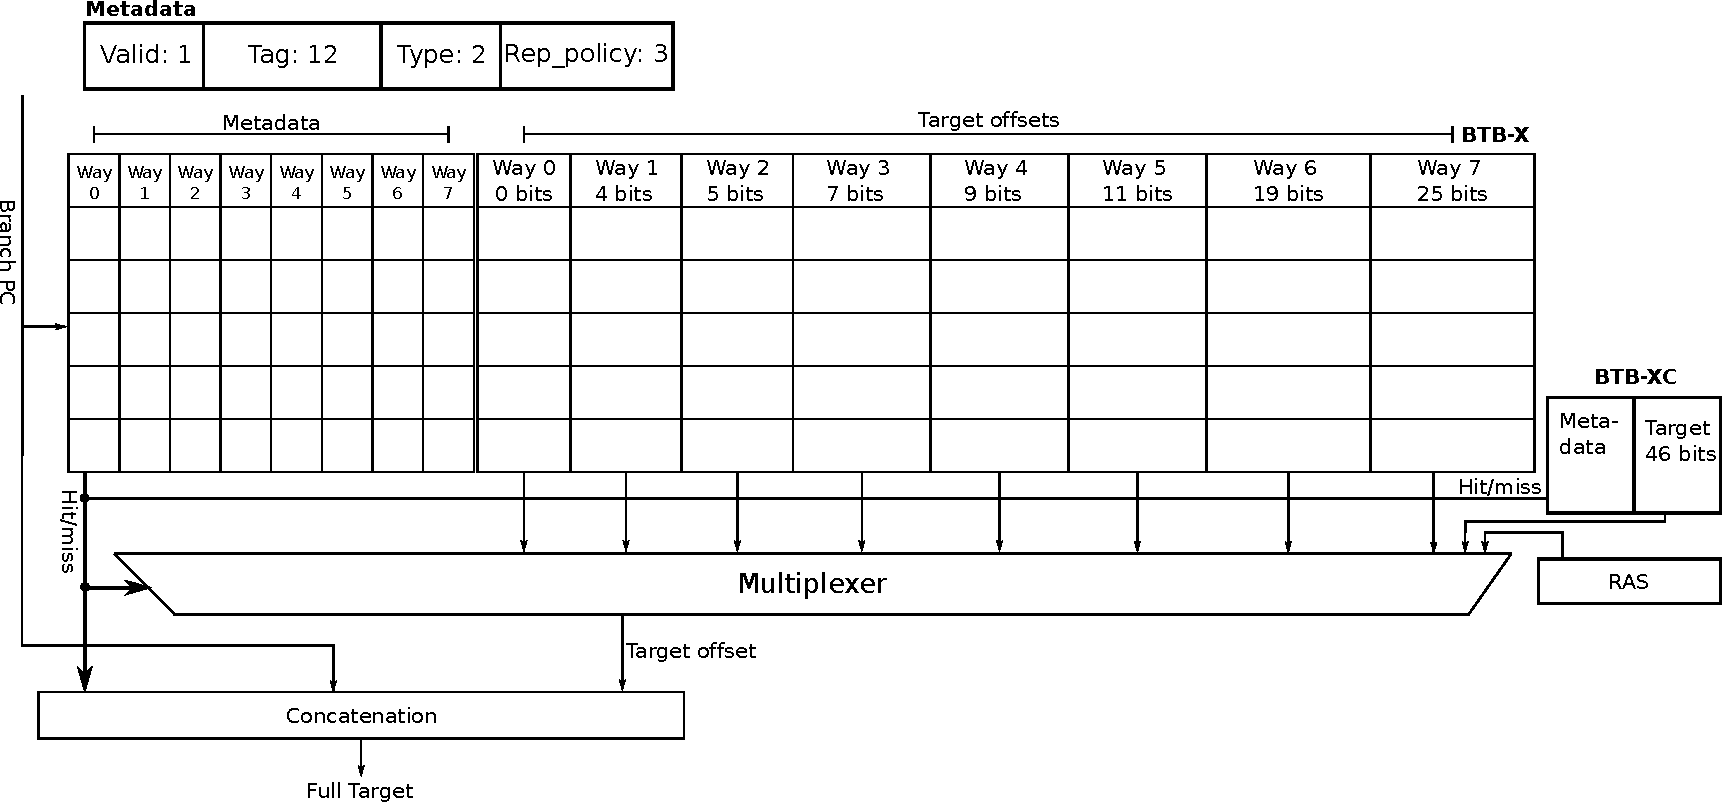
\includegraphics[width=\textwidth]{figures/BTB-X.pdf}
  \caption{\label{fig:btbx-design} The design of BTB-X.}
\end{figure}

Based on this observation we propose BTB-X, a reorganized BTB that
uses differently sized ways matching the distribution of target offset
sizes that we observed. The full design of BTB-X is shown in
\Cref{fig:btbx-design}. To accommodate branch targets that require the
full address size, we use a small conventional BTB called BTB-XC. When
accessing the BTB, BTB-X and BTB-XC are looked up in
parallel. Performing a BTB-X lookup is similar to performing a lookup
in a conventional BTB. The key difference is that the BTB-X lookup
yields a target offset rather than the full target address. Thus, the
target offset must be concatenated with the branch PC to obtain the
full target address. When allocating an entry, BTB-X stores the target
offset in the first free way where it will fit.

We implement and evaluate BTB-X using the Champsim simulator. Champsim
is a trace-based simulator used for for microarchitectural
studies~\cite{champsim}. For evaluation we use the aforementioned
workload traces released as part of the \liningfigures{IPC-1} championship. The traces
were provided by Qualcomm and include both server and client
workloads. For the BTB-X design to be applicable to all workloads, the
branch target offset size distribution that guided its design must be
shown to be widely applicable. To ensure this, we measure the branch
target offset size distributions of the more than 750 traces provided
by Qualcomm as part of the First Championship Value Prediction \liningfigures{CVP-1}
and traces from 6 known server applications. These results show nearly
identical branch target offset size distributions.
Finally, we measure the energy requirements and access latencies of
BTB-X, the state-of-the-art BTB design and a conventional BTB using Cacti 7.0~\cite{cacti} at the 22nm technology node.

\paragraph{Key Results.}

Our evaluation shows that BTB-X stores 2.24\texttimes{} more branches
than a conventional BTB organization. Furthermore, when compared to
the state of the art BTB design PDede, BTB-X stores  and
1.24\texttimes{} and 1.34\texttimes{} more branches for storage budgets of
0.9KB and 59KB respectively. This increase in branch storage density
translates to a significant decrease in BTB MPKI. Specifically, BTB-X lowers BTB MPKI to 9.3 compared to 25 for a conventional BTB. When looking at the overall performance gain of introducing an FDIP instruction prefetcher using different BTB configurations we see that FDIP produces geomean speedups of 24\%, 33\% and 38\% respectively for Conv-BTB, PDede and BTB-X respectively. Estimates of the power requirements of BTB-X show that reading and writing require 8.5~pJ and 11.4~pJ respectively. This compares favorably to the up to 9.4~pJ and 19.5~pJ respectively required by PDede and 13.2~pJ 25.2~pJ by Conv-BTB respectively. The access latency of BTB-X is 0.33~ns compared to 0.36~ns and 0.47~ms for Conv-BTB and PDede respectively.

We see that BTB-X outperforms the state of the art BTB organization PDede while, at the same time, proposes a simpler design that avoids BTB access indirections.


% \truls{Emphasize how the evaluation methodology using the traces from server workloads applies to FaaS workloads since a) they are fundamentally similar except that FaaS workloads run for a shorter time and b) we and prior work shows that FaaS workloads also have a large code footprint}

\subsection{Research direciton B: Software optimizations for serverless computing}

\paragraph{Motivation.}
The network-backed RPC interfaces commonly use to facilitate
inter-function communications in FaaS applications are a key
facilitator of the loose coupling between functions that give FaaS
many of its attractive
benefits~\cite{gan19_open_sourc_bench_suite_micros}. The RPC
interfaces allow FaaS functions written in different languages to
communicate with each other and it allows functions to be swapped out
at runtime as long as their external interfaces is
preserved. Furthermore, since RPC protocols can use a networked
transport, FaaS functions communicating over RPC can be transparently
distributed across physical nodes. The major disadvantage of these
network-backed RPC interlaces is that they induce a massive
inter-function communication latency. Where the latency of a local
function call in a monolith application is in the order of a new
nanoseconds, RPC-backed function calls between FaaS functions in a
FaaS application can take several milliseconds to execute -- a
difference of several orders of magnitude. When two FaaS functions
scheduled for execution on different nodes need to communicate, using
a networked RPC interface for communication is necessary. However,
when two FaaS functions are scheduled on the same node, using the RPC
interface for communication only adds overhead without giving any
benefits. To tackle this issue, prior work has proposed diverse
mechanisms aiming to reduce the inter-function communication overhead
of FaaS \cite{kotni21_faast,
  mahgoub22_wisef,barcelona-pons19_faas_track,sreekanti20_cloud,shillaker20_faasm,jia21_night}.
Common for all of these approaches, however, is that they violate one
or more of the key properties of FaaS that makes the programming model
attractive to developers (see \Cref{sec:serverless}).


\begin{figure}[ht]
  \centering
  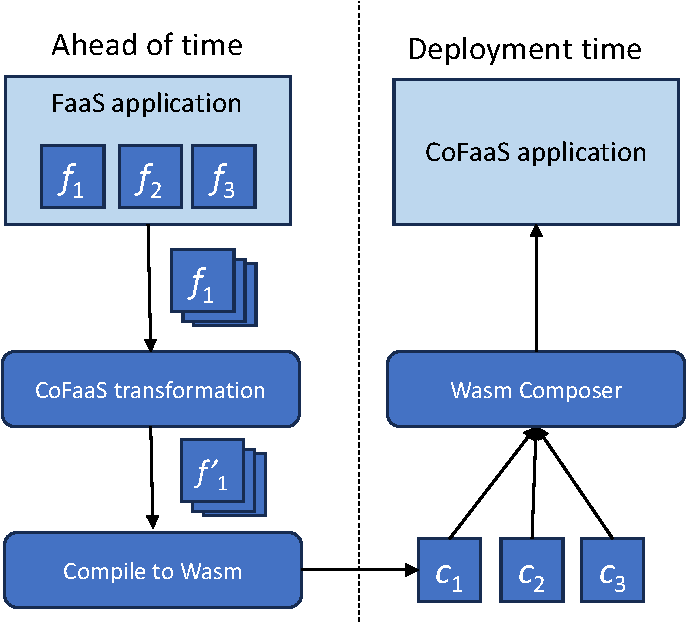
\includegraphics[width=0.5\textwidth]{papers/paper5-cofaas/figures/cofaas_compilation.pdf}
  \caption{\label{fig:cofaas-comp} The compilation workflow required when using CoFaaS.}
\end{figure}


\paragraph{Approach.}
We propose CoFaaS, a software transformation of FaaS applications that eliminate the inter-function communication overhead. CoFaaS is unique in the landscape as it eliminates the FaaS communication overhead without sacrificing any of the key properties that makes FaaS attractive to developers. The CoFaaS transformation is fully automatic and can be applied to existing FaaS applications without requiring manual modification of existing functions.


For FaaS functions to communicate, their public interfaces must be
specified using language-independent Interface Definition Languages
(IDL). For example, a popular used IDL in FaaS applications is
Protobuf. The IDL definitions written in Protobuf~\cite{protobuf} are
used by Google's gRPC~\cite{grpc} framework. CoFaaS makes the key
insight that, is that as long as we keep the public interface
unchanged, we can transform the function implementation
freely. Furthermore, since IDLs are declarative, they can be easily
mapped to other IDLs. We exploit this to retarget FaaS functions run
on a single WebAssembly (Wasm)~\cite{rossberg22_webas_core_specif}
runtime. Wasm is a language-independent portable bytecode format with
wide platform support. In order for the FaaS functions to co-exist on
a single Wasm runtime, we transform the FaaS functions into a Wasm
component. Wasm components~\cite{compmodel}, like FaaS functions, use
a language-independent IDL to define their public interface and since
each Wasm component exist in their own isolated memory space, we can
simply transform the IDL of the FaaS function to the IDL of Wasm and
compile the functions to Wasm. The final point to address is that the
original functions are written to communicate over a network-backed
RPC interface. To address this we do two things: First, we provide a
stub library that provides API-level compatibility with the original
gRPC library but instead of calling other functions using a networked
RPC call, it uses the Wasm interface to call functions running on the
same Wasm runtime.

For evaluating CoFaaS we use a two-function producer-consumer FaaS
application that works as follows: A client issues a request to the
producer function, then the producer function generates a data payload
of $m$ bytes and transmits this payload to the consumer
function. Finally, the request from the producer to the consumer is
repeated $n$ times. By changing values for $m$ and $n$ evaluation we
are able to estimate \begin{inparaenum}[a)]
\item to what extent the latency reduction CoFaaS achieves is
  amortized by the data transfer happening between the consumer and
  producer and \item we can estimate the impact of CoFaaS on more
  complex applications consisting of more functions by varying the
  number of intra-application requests.
\end{inparaenum} We compare two versions of the application, one written in Go and one written in Rust.


\paragraph{Key Results.}
We evaluate CoFaaS using a two-function FaaS application that CoFaaS
reduces the round-trip request time of the FaaS application that we
evaluate by 6\texttimes. For a 1 kilobyte payload, the latency of
inter-function requests is reduced by up to 100\texttimes. For larger
payload sizes, the achieved speedup diminishes but remains
significant, with a 2\texttimes{} speedup being achieved for the largest
evaluated payload size of 512 kilobytes. We note that the median
inter-function request payload size observed in real-world FaaS traces
is 8 kilobytes~\cite{mahgoub22_wisef}. For this size, CoFaaS gives a
20\texttimes{} speedup. Further, the round-trip time speedup increases
when we increase the number of intra-application requests. This
indicates that the relative advantage of CoFaaS is bigger for more
complex applications.

Introducing CoFaaS in a production environment adds only minimal
overhead. This is because transforming a FaaS function to a composable
CoFaaS component is simply another compilation step. The operation
needed to compose CoFaaS components into an application is
instantaneous and can easily be done at deployment time. The process
of applying the CoFaaS transformation to a FaaS application is shown
in \Cref{fig:cofaas-comp}.

%\subsection{Primary contribution 2: 

\ifx\chapincluded\undefined
  \printbibliography
  \end{refsection}
 \fi
\end{document}


%%% Local Variables:
%%% mode: latex
%%% TeX-master: t
%%% TeX-command-extra-options: "-shell-escape"
%%% End: